\documentclass[border=5pt]{standalone}
\usepackage[utf8]{inputenc}
\usepackage{amsmath}
\usepackage{amssymb}

\usepackage{tikz}
\usetikzlibrary{shapes.geometric, arrows}

\tikzstyle{startstop} = [rectangle, rounded corners, minimum width=3cm, minimum height=1cm,text centered, draw=black, fill=red!30]
\tikzstyle{io} = [trapezium, trapezium left angle=70, trapezium right angle=110, minimum width=3cm, minimum height=1cm, text centered, draw=black, fill=blue!30]
\tikzstyle{process} = [rectangle, minimum width=3cm, minimum height=1cm, text centered, draw=black, fill=orange!30]
\tikzstyle{decision} = [diamond, minimum width=3cm, minimum height=1cm, text centered, draw=black, fill=green!30]
\tikzstyle{arrow} = [thick,->,>=stealth, rounded corners]
\tikzstyle{fdot} = [circle, minimum width=4pt, fill]
\tikzstyle{line} = [thick,>=stealth, rounded corners]

\begin{document}

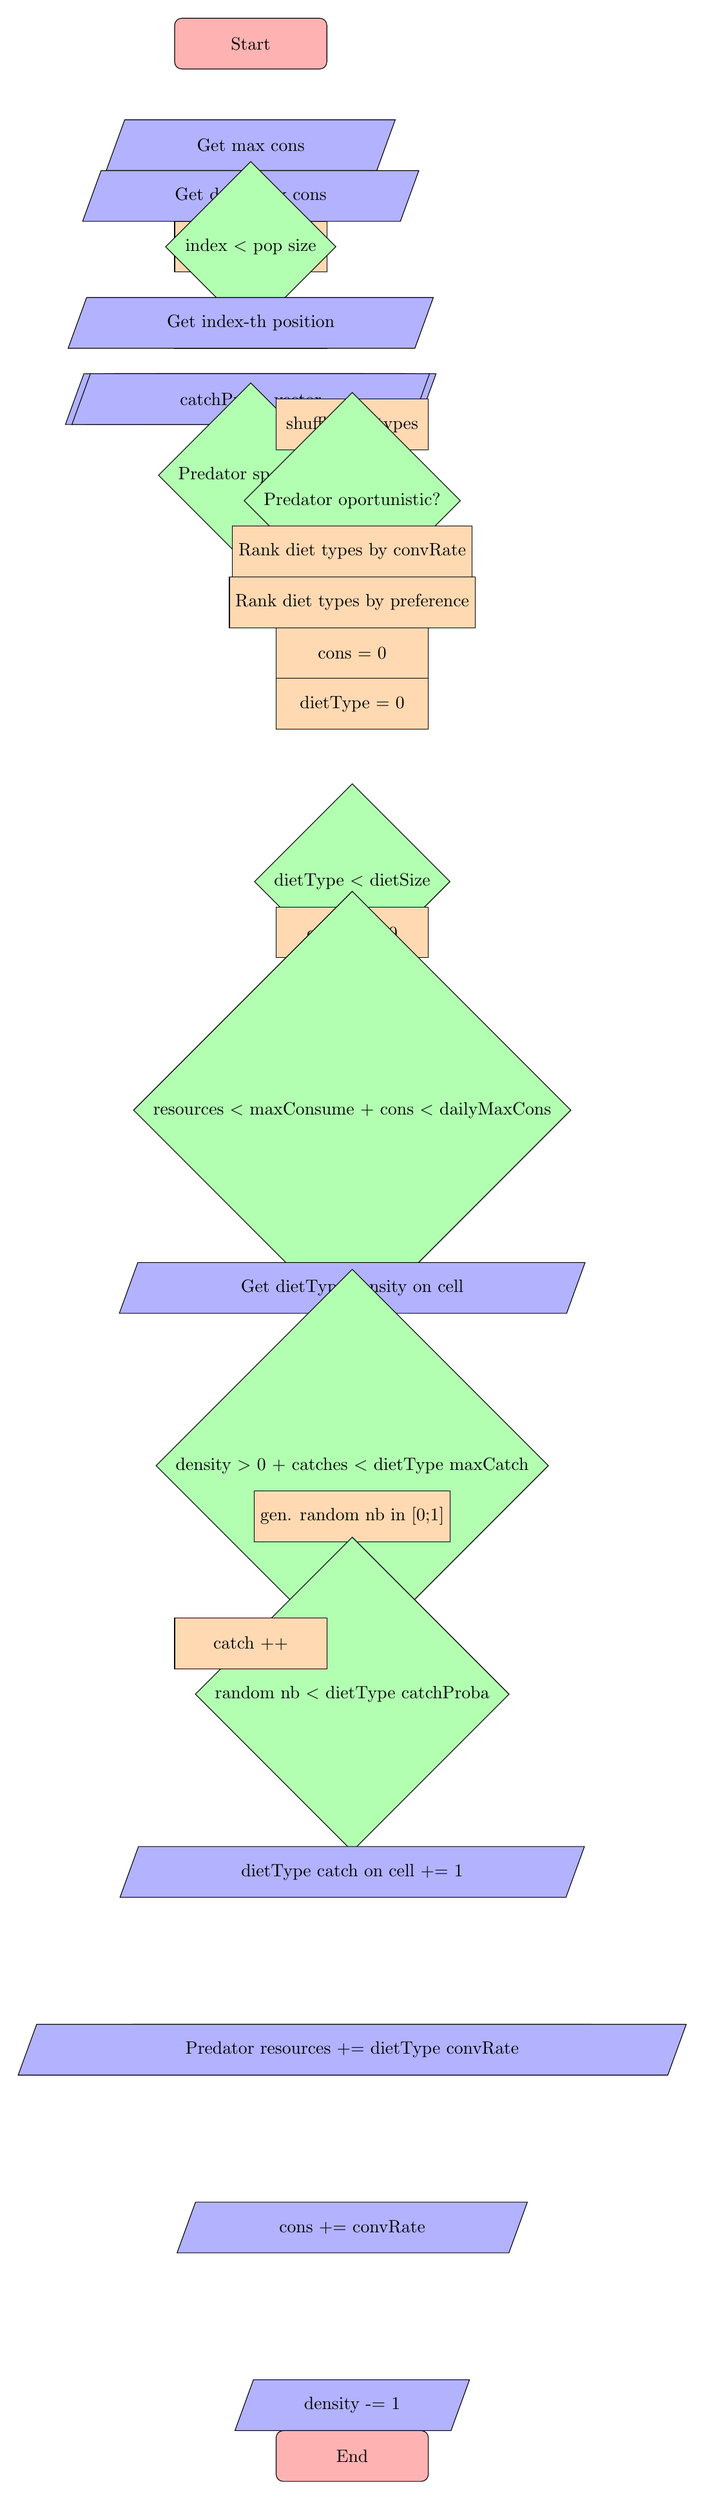
\begin{tikzpicture}[node distance=2cm]

\node (start) [startstop] {Start};
\node (in1) [io, below of=start] {Get max cons};
\node (in2) [io, below of=in1, yshift=1cm] {Get daily max cons};
\node (pro1) [process, below of=in2, yshift=1cm] {Shuffle pop table};
\node (pro2) [process, below of=pro1, yshift=0.5cm] {index = 0};
\node (dec1) [decision, below of=in1] {index $<$ pop size};
\node (in3) [io, below of=dec1, yshift=0.5cm] {Get index-th position};
\node (in4) [io, below of=in3, yshift=0.5cm] {Resources};
\node (in5) [io, below of=in3, yshift=0.5cm] {Get diet vector};
\node (in6) [io, below of=in3, yshift=0.5cm] {convRate vector};
\node (in7) [io, below of=in3, yshift=0.5cm] {maxCatches vector};
\node (in8) [io, below of=in3, yshift=0.5cm] {catchProba vector};
\node (dec2) [decision, below of=in8, yshift=0.5cm] {Predator specific ?};
\node (pro3) [process, right of=dec2, yshift=1cm] {shuffle diet types};
\node (dec3) [decision, below of=pro3, yshift=0.5cm] {Predator oportunistic?};
\node (pro4) [process, below of=dec3, yshift=1cm] {Rank diet types by convRate};
\node (pro5) [process, below of=pro4, yshift=1cm] {Rank diet types by preference};
\node (pro6) [process, below of=pro5, yshift=1cm] {cons = 0};
\node (pro7) [process, below of=pro6, yshift=1cm] {dietType = 0};
\node (dec4) [decision, below of=pro7, yshift=-1.5cm] {dietType $<$ dietSize};
\node (pro8) [process, below of=dec4, yshift=1cm] {catches = 0};
\node (dec5) [decision, below of=pro8, yshift=-1.5cm] {resources $<$ maxConsume + cons $<$ dailyMaxCons};
\node (in9) [io, below of=dec5, yshift=-1.5cm] {Get dietType density on cell};
\node (dec6) [decision, below of=in9, yshift=-1.5cm] {density $>$ 0 + catches $<$ dietType maxCatch};
\node (pro9) [process, below of=dec6, yshift=1cm] {gen. random nb in [0;1]};
\node (dec7) [decision, below of=pro9, yshift=-1.5cm] {random nb $<$ dietType catchProba};
\node (pro10) [process, left of=dec7, yshift=1cm] {catch ++};
\node (out1) [io, below of=dec7, yshift=-1.5cm] {dietType catch on cell += 1};
\node (out2) [io, below of=out1, yshift=-1.5cm] {dietType density on cell -= 1};
\node (out3) [io, below of=out1, yshift=-1.5cm] {Predator resources += dietType convRate};
\node (out4) [io, below of=out3, yshift=-1.5cm] {cons += convRate};
\node (out5) [io, below of=out4, yshift=-1.5cm] {density -= 1};
\node (stop) [startstop, below of=out5, yshift=1cm] {End};

%\draw [arrow] (start) -- (pro1);
%\draw [arrow] (pro1) -- (dec1);
%\draw [arrow] (dec1) -- node[anchor=east] {yes} (in1);
%\draw [arrow] (dec1) -| node[anchor=south, xshift=-4cm] {no} + (6,-0.5) |- (stop);
%\draw [arrow] (in1) -- (dec2);
%\draw [arrow] (dec2) -- node[anchor=east] {yes} (pro2);
%\draw [line] (dec2) -| node[anchor=south, xshift=-3.5cm] {no} + (5.5,-0.5) |- (pro5);
%\draw [arrow] (pro2) -- (pro3);
%\draw [arrow] (pro3) -- (dec3);
%\draw [arrow] (dec3) -- node[anchor=east] {yes} (in2);
%\draw [arrow] (dec3) -- node[anchor=south, xshift=0cm] {no} + (5.5,0) |- (pro5);
%\draw [arrow] (in3) -- (dec4);
%\draw [arrow] (dec4) -- node[anchor=east] {yes} (out1);
%\draw [arrow] (dec4) -- node[anchor=south, xshift=0cm] {no} + (5,0) |- (pro4);
%\draw [arrow] (out1) -- (pro4);
%\draw [arrow] (pro4) -| + (-5.5,0) |- (dec2);
%\draw [arrow] (pro5) -| + (-6,0) |- (dec1);

\end{tikzpicture}

\end{document}